\chapter{HTTP and Forms}\label{http}

\epigraphhead[30]{
\epigraph{\hspace*{-.1cm}\itshape``Communication must be stateless in nature [...] such that each request from client to server must contain all of the information necessary to understand the request, and cannot take advantage of any stored context on the server.''}%
{---Roy Fielding, Architectural Styles and the Design of Network-based Software Architectures}
}\index{Fielding, Roy}\index{browser!environment}

The \emph{Hypertext Transfer Protocol}, already mentioned in \hyperref[browser.web]{Chapter 13}, is the mechanism through which data is requested and provided on the \index{World Wide Web}World Wide Web. This chapter describes the \index{protocol}protocol in more detail and explains the way browser JavaScript has access to it.

\section{The protocol}\index{IP address}

If you type \emph{eloquentjavascript.net\slash 18\_http.html} into your browser's \index{address bar}address bar, the \index{browser}browser first looks up the \index{address}address of the server associated with \emph{eloquentjavascript.net} and tries to open a \index{TCP}TCP \index{connection}connection to it on \index{port}port 80, the default port for \index{HTTP}HTTP traffic. If the \index{server}server exists and accepts the connection, the browser might send something like this:

\begin{lstlisting}
GET /18_http.html HTTP/1.1
Host: eloquentjavascript.net
User-Agent: Your browser's name
\end{lstlisting}
\noindent

Then the server responds, through that same connection.

\begin{lstlisting}
HTTP/1.1 200 OK
Content-Length: 65585
Content-Type: text/html
Last-Modified: Mon, 08 Jan 2018 10:29:45 GMT

<!doctype html>
... the rest of the document
\end{lstlisting}
\noindent

The browser takes the part of the \index{response}response after the blank line, its \emph{body} (not to be confused with the HTML \lstinline`<body>` tag), and displays it as an \index{HTML}HTML document.\index{HTTP}

The information sent by the client is called the \emph{\index{request}request}. It starts with this line:

\begin{lstlisting}
GET /18_http.html HTTP/1.1
\end{lstlisting}
\noindent\index{DELETE method}\index{PUT method}\index{GET method}\index{method!HTTP}

The first word is the \emph{method} of the \index{request}request. \lstinline`GET` means that we want to \emph{get} the specified resource. Other common methods are \lstinline`DELETE` to delete a resource, \lstinline`PUT` to create or replace it, and \lstinline`POST` to send information to it. Note that the \index{server}server is not obliged to carry out every request it gets. If you walk up to a random website and tell it to \lstinline`DELETE` its main page, it'll probably refuse.\index{path!URL}\index{GitHub}\index{file!resource}

The part after the method name is the path of the \emph{\index{resource}resource} the request applies to. In the simplest case, a resource is simply a file on the \index{server}server, but the protocol doesn't require it to be. A resource may be anything that can be transferred \emph{as if} it is a file. Many servers generate the responses they produce on the fly. For example, if you open \href{https://github.com/marijnh}{\emph{https://github.com\slash marijnh}}, the server looks in its database for a user named ``marijnh'', and if it finds one, it will generate a profile page for that user.

After the resource path, the first line of the request mentions \lstinline`HTTP/1.1` to indicate the \index{version}version of the \index{HTTP}HTTP \index{protocol}protocol it is using.

In practice, many sites use HTTP version 2, which supports the same concepts as version 1.1 but is a lot more complicated so that it can be faster. Browsers will automatically switch to the appropriate protocol version when talking to a given server, and the outcome of a request is the same regardless of which version is used. Because version 1.1 is more straightforward and easier to play around with, we'll focus on that.\index{status code}

The server's \index{response}response will start with a version as well, followed by the status of the response, first as a three-digit status code and then as a human-readable string.

\begin{lstlisting}
HTTP/1.1 200 OK
\end{lstlisting}
\noindent\index{200 (HTTP status code)}\index{error response}\index{404 (HTTP status code)}

Status codes starting with a 2 indicate that the request succeeded. Codes starting with 4 mean there was something wrong with the \index{request}request. 404 is probably the most famous HTTP status code—it means that the resource could not be found. Codes that start with 5 mean an error happened on the \index{server}server and the request is not to blame.\index{HTTP}

\label{http.headers}The first line of a request or response may be followed by any number of \emph{\index{header}headers}. These are lines in the form \lstinline`name: value` that specify extra information about the request or response. These headers were part of the example \index{response}response:

\begin{lstlisting}
Content-Length: 65585
Content-Type: text/html
Last-Modified: Thu, 04 Jan 2018 14:05:30 GMT
\end{lstlisting}
\noindent\index{Content-Length header}\index{Content-Type header}\index{Last-Modified header}

This tells us the size and type of the response document. In this case, it is an HTML document of 65,585 bytes. It also tells us when that document was last modified.\index{Host header}\index{domain}

For most \index{header}headers, the client and server are free to decide whether to include them in a \index{request}request or \index{response}response. But a few are required. For example, the \lstinline`Host` header, which specifies the hostname, should be included in a request because a \index{server}server might be serving multiple hostnames on a single \index{IP address}IP address, and without that header, the server won't know which hostname the client is trying to talk to.\index{GET method}\index{DELETE method}\index{PUT method}\index{POST method}\index{body (HTTP)}

After the headers, both requests and responses may include a blank line followed by a body, which contains the data being sent. \lstinline`GET` and \lstinline`DELETE` requests don't send along any data, but \lstinline`PUT` and \lstinline`POST` requests do. Similarly, some response types, such as error responses, do not require a body.

\section{Browsers and HTTP}\index{HTTP}\index{file!resource}

As we saw in the example, a \index{browser}browser will make a request when we enter a \index{URL}URL in its \index{address bar}address bar. When the resulting HTML page references other files, such as \index{image}images and JavaScript files, those are also retrieved.\index{parallelism}\index{GET method}

A moderately complicated \index{website}website can easily include anywhere from 10 to 200 \index{resource}resources. To be able to fetch those quickly, browsers will make several \lstinline`GET` requests simultaneously, rather than waiting for the responses one at a time.

HTML pages may include \emph{\index{form}forms}, which allow the user to fill out information and send it to the server. This is an example of a form:

\begin{lstlisting}
<form method="GET" action="example/message.html">
  <p>Name: <input type="text" name="name"></p>
  <p>Message:<br><textarea name="message"></textarea></p>
  <p><button type="submit">Send</button></p>
</form>
\end{lstlisting}
\noindent\index{form}\index{method attribute}\index{GET method}

This code describes a form with two \index{field}fields: a small one asking for a name and a larger one to write a message in. When you click the Send \index{button}button, the form is \emph{submitted}, meaning that the content of its field is packed into an HTTP request and the browser navigates to the result of that request.

When the \lstinline`<form>` element's \lstinline`method` attribute is \lstinline`GET` (or is omitted), the information in the form is added to the end of the \lstinline`action` URL as a \emph{\index{query string}query string}. The browser might make a request to this URL:

\begin{lstlisting}
GET /example/message.html?name=Jean&message=Yes%3F HTTP/1.1
\end{lstlisting}
\noindent\index{ampersand character}

The \index{question mark}question mark indicates the end of the path part of the URL and the start of the query. It is followed by pairs of names and values, corresponding to the \lstinline`name` attribute on the form field elements and the content of those elements, respectively. An ampersand character (\lstinline`&`) is used to separate the pairs.\index{escaping!in URLs}\index{hexadecimal number}\index{encodeURIComponent function}\index{decodeURIComponent function}

The actual message encoded in the URL is ``Yes?'', but the question mark is replaced by a strange code. Some characters in query strings must be escaped. The question mark, represented as \lstinline`%3F`, is one of those. There seems to be an unwritten rule that every format needs its own way of escaping characters. This one, called \emph{\index{URL encoding}URL encoding}, uses a \index{percent sign}percent sign followed by two hexadecimal (base 16) digits that encode the character code. In this case, 3F, which is 63 in decimal notation, is the code of a question mark character. JavaScript provides the \lstinline`encodeURIComponent` and \lstinline`decodeURIComponent` functions to encode and decode this format.

\begin{lstlisting}
console.log(encodeURIComponent("Yes?"));
// → Yes%3F
console.log(decodeURIComponent("Yes%3F"));
// → Yes?
\end{lstlisting}
\noindent\index{body (HTTP)}\index{POST method}

If we change the \lstinline`method` attribute of the HTML form in the example we saw earlier to \lstinline`POST`, the \index{HTTP}HTTP request made to submit the \index{form}form will use the \lstinline`POST` method and put the \index{query string}query string in the body of the request, rather than adding it to the URL.

\begin{lstlisting}
POST /example/message.html HTTP/1.1
Content-length: 24
Content-type: application/x-www-form-urlencoded

name=Jean&message=Yes%3F
\end{lstlisting}
\noindent

\lstinline`GET` requests should be used for requests that do not have \index{side
effect}side
effects but simply ask for information. Requests that change something on the server, for example creating a new account or posting a message, should be expressed with other methods, such as \lstinline`POST`. Client-side software such as a browser knows that it shouldn't blindly make \lstinline`POST` requests but will often implicitly make \lstinline`GET` requests—for example to prefetch a resource it believes the user will soon need.

We'll come back to forms and how to interact with them from JavaScript \hyperref[http.forms]{later in the chapter}.

\label{http.fetch}\section{Fetch}\index{fetch function}\index{Promise class}\index{interface!module}

The interface through which browser JavaScript can make HTTP requests is called \lstinline`fetch`. Since it is relatively new, it conveniently uses promises (which is rare for browser interfaces).

\begin{lstlisting}
fetch("example/data.txt").then(response => {
  console.log(response.status);
  // → 200
  console.log(response.headers.get("Content-Type"));
  // → text/plain
});
\end{lstlisting}
\noindent\index{Response class}\index{status property}\index{headers property}

Calling \lstinline`fetch` returns a promise that resolves to a \lstinline`Response` object holding information about the server's response, such as its status code and its headers. The headers are wrapped in a \lstinline`Map`-like object that treats its keys (the header names) as case insensitive because header names are not supposed to be case sensitive. This means \lstinline`headers.get("Content-Type")` and \lstinline`headers.get("content-TYPE")` will return the same value.

Note that the promise returned by \lstinline`fetch` resolves successfully even if the server responded with an error code. It \emph{might} also be rejected if there is a network error or if the \index{server}server that the request is addressed to can't be found.\index{path!URL}\index{relative URL}

The first argument to \lstinline`fetch` is the URL that should be requested. When that \index{URL}URL doesn't start with a protocol name (such as \emph{http:}), it is treated as \emph{relative}, which means it is interpreted relative to the current document. When it starts with a slash (/), it replaces the current path, which is the part after the server name. When it does not, the part of the current path up to and including its last \index{slash character}slash character is put in front of the relative URL.\index{text method}\index{body (HTTP)}\index{Promise class}

To get at the actual content of a response, you can use its \lstinline`text` method. Because the initial promise is resolved as soon as the response's headers have been received and because reading the response body might take a while longer, this again returns a promise.

\begin{lstlisting}
fetch("example/data.txt")
  .then(resp => resp.text())
  .then(text => console.log(text));
// → This is the content of data.txt
\end{lstlisting}
\noindent\index{json method}

A similar method, called \lstinline`json`, returns a promise that resolves to the value you get when parsing the body as \index{JSON}JSON or rejects if it's not valid JSON.\index{GET method}\index{body (HTTP)}\index{DELETE method}\index{method property}

By default, \lstinline`fetch` uses the \lstinline`GET` method to make its request and does not include a request body. You can configure it differently by passing an object with extra options as a second argument. For example, this request tries to delete \lstinline`example/data.txt`:

\begin{lstlisting}
fetch("example/data.txt", {method: "DELETE"}).then(resp => {
  console.log(resp.status);
  // → 405
});
\end{lstlisting}
\noindent\index{405 (HTTP status code)}

The 405 status code means ``method not allowed'', an HTTP server's way of saying ``I can't do that''.\index{Range header}\index{body property}\index{headers property}

To add a request body, you can include a \lstinline`body` option. To set headers, there's the \lstinline`headers` option. For example, this request includes a \lstinline`Range` header, which instructs the server to return only part of a response.

\begin{lstlisting}
fetch("example/data.txt", {headers: {Range: "bytes=8-19"}})
  .then(resp => resp.text())
  .then(console.log);
// → the content
\end{lstlisting}
\noindent

The browser will automatically add some request \index{header}headers, such as ``Host'' and those needed for the server to figure out the size of the body. But adding your own headers is often useful to include things such as authentication information or to tell the server which file format you'd like to receive.

\label{http.http_sandbox}\section{HTTP sandboxing}\index{sandbox}\index{browser!security}

Making \index{HTTP}HTTP requests in web page scripts once again raises concerns about \index{security}security. The person who controls the script might not have the same interests as the person on whose computer it is running. More specifically, if I visit \emph{themafia.org}, I do not want its scripts to be able to make a request to \emph{mybank.com}, using identifying information from my browser, with instructions to transfer all my money to some random account.

For this reason, browsers protect us by disallowing scripts to make HTTP requests to other \index{domain}domains (names such as \emph{themafia.org} and \emph{mybank.com}).\index{Access-Control-Allow-Origin header}\index{cross-domain request}

This can be an annoying problem when building systems that want to access several domains for legitimate reasons. Fortunately, \index{server}servers can include a \index{header}header like this in their \index{response}response to explicitly indicate to the browser that it is okay for the request to come from another domain:

\begin{lstlisting}
Access-Control-Allow-Origin: *
\end{lstlisting}
\noindent

\section{Appreciating HTTP}\index{client}\index{HTTP}\index{interface!HTTP}

When building a system that requires \index{communication}communication between a JavaScript program running in the \index{browser}browser (client-side) and a program on a \index{server}server (server-side), there are several different ways to model this communication.\index{network!abstraction}\index{abstraction}

A commonly used model is that of \emph{\index{remote procedure call}remote procedure calls}. In this model, communication follows the patterns of normal function calls, except that the function is actually running on another machine. Calling it involves making a request to the server that includes the function's name and arguments. The response to that request contains the returned value.

When thinking in terms of remote procedure calls, HTTP is just a vehicle for communication, and you will most likely write an abstraction layer that hides it entirely.\index{media type}\index{document format}\index{method!HTTP}

Another approach is to build your communication around the concept of \index{resource}resources and \index{HTTP}HTTP methods. Instead of a remote procedure called \lstinline`addUser`, you use a \lstinline`PUT` request to \lstinline`/users/larry`. Instead of encoding that user's properties in function arguments, you define a JSON document format (or use an existing format) that represents a user. The body of the \lstinline`PUT` request to create a new resource is then such a document. A resource is fetched by making a \lstinline`GET` request to the resource's URL (for example, \lstinline`/user/larry`), which again returns the document representing the resource.

This second approach makes it easier to use some of the features that HTTP provides, such as support for caching resources (keeping a copy on the client for fast access). The concepts used in HTTP, which are well designed, can provide a helpful set of principles to design your server interface around.

\section{Security and HTTPS}\index{man-in-the-middle}\index{security}\index{HTTPS}\index{network!security}

Data traveling over the Internet tends to follow a long, dangerous road. To get to its destination, it must hop through anything from coffee shop Wi-Fi hotspots to networks controlled by various companies and states. At any point along its route it may be inspected or even modified.\index{tampering}

If it is important that something remain secret, such as the \index{password}password to your \index{email}email account, or that it arrive at its destination unmodified, such as the account number you transfer money to via your bank's website, plain HTTP is not good enough.\index{cryptography}\index{encryption}\index{Secure HTTP|see{HTTPS}}

The secure \index{HTTP}HTTP protocol, used for \index{URL}URLs starting with \emph{https://}, wraps HTTP traffic in a way that makes it harder to read and tamper with. Before exchanging data, the client verifies that the server is who it claims to be by asking it to prove that it has a cryptographic \index{certificate}certificate issued by a certificate authority that the browser recognizes. Next, all data going over the \index{connection}connection is encrypted in a way that should prevent eavesdropping and tampering.

Thus, when it works right, \index{HTTPS}HTTPS prevents other people from impersonating the website you are trying to talk to and from snooping on your communication. It is not perfect, and there have been various incidents where HTTPS failed because of forged or stolen certificates and broken software, but it is a \emph{lot} safer than plain HTTP.

\label{http.forms}\section{Form fields}

Forms were originally designed for the pre-JavaScript Web to allow web sites to send user-submitted information in an HTTP request. This design assumes that interaction with the server always happens by navigating to a new page.\index{DOM!fields}

But their elements are part of the DOM like the rest of the page, and the DOM elements that represent form \index{field}fields support a number of properties and events that are not present on other elements. These make it possible to inspect and control such input fields with JavaScript programs and do things such as adding new functionality to a form or using forms and fields as building blocks in a JavaScript application.\index{form (HTML tag)}

A web form consists of any number of input \index{field}fields grouped in a \lstinline`<form>` tag. HTML allows several different styles of fields, ranging from simple on\slash off checkboxes to drop-down menus and fields for text input. This book won't try to comprehensively discuss all field types, but we'll start with a rough overview.\index{input (HTML tag)}\index{type attribute}

A lot of field types use the \lstinline`<input>` tag. This tag's \lstinline`type` attribute is used to select the field's style. These are some commonly used \lstinline`<input>` types:\index{password field}\index{checkbox}\index{radio button}\index{file field}

\noindent\begin{tabular}{ll}
\lstinline`text` &
A single-line \index{text field}text field
\tabularnewline
\lstinline`password` &
Same as \lstinline`text` but hides the text that is typed
\tabularnewline
\lstinline`checkbox` &
An on\slash off switch
\tabularnewline
\lstinline`radio` &
(Part of) a \index{multiple-choice}multiple-choice field
\tabularnewline
\lstinline`file` &
Allows the user to choose a file from their computer
\tabularnewline
\end{tabular}\index{value attribute}\index{checked attribute}\index{form (HTML tag)}

Form fields do not necessarily have to appear in a \lstinline`<form>` tag. You can put them anywhere in a page. Such form-less fields cannot be \index{submit}submitted (only a form as a whole can), but when responding to input with JavaScript, we often don't want to submit our fields normally anyway.

\begin{lstlisting}
<p><input type="text" value="abc"> (text)</p>
<p><input type="password" value="abc"> (password)</p>
<p><input type="checkbox" checked> (checkbox)</p>
<p><input type="radio" value="A" name="choice">
   <input type="radio" value="B" name="choice" checked>
   <input type="radio" value="C" name="choice"> (radio)</p>
<p><input type="file"> (file)</p>
\end{lstlisting}
\noindent

The fields created with this HTML code look like this:

\vskip 1.5ex
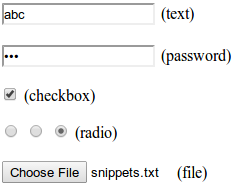
\includegraphics[width=4cm]{img/form_fields.png}
\vskip 1.5ex

The JavaScript interface for such elements differs with the type of the element.\index{textarea (HTML tag)}\index{text field}

Multiline text fields have their own tag, \lstinline`<textarea>`, mostly because using an attribute to specify a multiline starting value would be awkward. The \lstinline`<textarea>` tag requires a matching \lstinline`</textarea>` closing tag and uses the text between those two, instead of the \lstinline`value` attribute, as starting text.

\begin{lstlisting}
<textarea>
one
two
three
</textarea>
\end{lstlisting}
\noindent\index{select (HTML tag)}\index{option (HTML tag)}\index{multiple choice}\index{drop-down menu}

Finally, the \lstinline`<select>` tag is used to create a field that allows the user to select from a number of predefined options.

\begin{lstlisting}
<select>
  <option>Pancakes</option>
  <option>Pudding</option>
  <option>Ice cream</option>
</select>
\end{lstlisting}
\noindent

Such a field looks like this:

\vskip 1.5ex
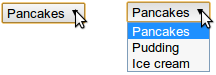
\includegraphics[width=4cm]{img/form_select.png}
\vskip 1.5ex\index{change event}

Whenever the value of a form field changes, it will fire a \lstinline`"change"` event.

\section{Focus}\index{keyboard}\index{focus}\index{keyboard focus|see{focus}}

Unlike most elements in HTML documents, form fields can get \emph{keyboard \index{focus}focus}. When clicked or activated in some other way, they become the currently active element and the recipient of keyboard \index{input}input.\index{option (HTML tag)}\index{select (HTML tag)}

Thus, you can type into a \index{text field}text field only when it is focused. Other fields respond differently to keyboard events. For example, a \lstinline`<select>` menu tries to move to the option that contains the text the user typed and responds to the arrow keys by moving its selection up and down.\index{focus method}\index{blur method}\index{activeElement property}

We can control \index{focus}focus from JavaScript with the \lstinline`focus` and \lstinline`blur` methods. The first moves focus to the DOM element it is called on, and the second removes focus. The value in \lstinline`document.activeElement` corresponds to the currently focused element.

\begin{lstlisting}
<input type="text">
<script>
  document.querySelector("input").focus();
  console.log(document.activeElement.tagName);
  // → INPUT
  document.querySelector("input").blur();
  console.log(document.activeElement.tagName);
  // → BODY
</script>
\end{lstlisting}
\noindent\index{autofocus attribute}

For some pages, the user is expected to want to interact with a form field immediately. JavaScript can be used to \index{focus}focus this field when the document is loaded, but HTML also provides the \lstinline`autofocus` attribute, which produces the same effect while letting the browser know what we are trying to achieve. This gives the browser the option to disable the behavior when it is not appropriate, such as when the user has put the focus on something else.\index{tab key}\index{keyboard}\index{tabindex attribute}\index{a (HTML tag)}

Browsers traditionally also allow the user to move the focus through the document by pressing the \textsc{tab} key. We can influence the order in which elements receive focus with the \lstinline`tabindex` attribute. The following example document will let the focus jump from the text input to the OK button, rather than going through the help link first:

\begin{lstlisting}
<input type="text" tabindex=1> <a href=".">(help)</a>
<button onclick="console.log('ok')" tabindex=2>OK</button>
\end{lstlisting}
\noindent\index{tabindex attribute}

By default, most types of HTML elements cannot be focused. But you can add a \lstinline`tabindex` attribute to any element that will make it focusable. A \lstinline`tabindex` of -1 makes tabbing skip over an element, even if it is normally focusable.

\section{Disabled fields}\index{disabled attribute}

All \index{form}form \index{field}fields can be \emph{disabled} through their \lstinline`disabled` attribute. It is an \index{attribute}attribute that can be specified without value—the fact that it is present at all disables the element.

\begin{lstlisting}
<button>I'm all right</button>
<button disabled>I'm out</button>
\end{lstlisting}
\noindent

Disabled fields cannot be \index{focus}focused or changed, and browsers make them look gray and faded.

\vskip 1.5ex

\includegraphics[width=3cm]{img/button_disabled.png}
\vskip 1.5ex\index{user experience}

When a program is in the process of handling an action caused by some \index{button}button or other control that might require communication with the server and thus take a while, it can be a good idea to disable the control until the action finishes. That way, when the user gets impatient and clicks it again, they don't accidentally repeat their action.

\section{The form as a whole}\index{array-like object}\index{form (HTML tag)}\index{form property}\index{elements property}

When a \index{field}field is contained in a \lstinline`<form>` element, its DOM element will have a \lstinline`form` property linking back to the form's DOM element. The \lstinline`<form>` element, in turn, has a property called \lstinline`elements` that contains an array-like collection of the fields inside it.\index{elements property}\index{name attribute}

The \lstinline`name` attribute of a form field determines the way its value will be identified when the form is \index{submit}submitted. It can also be used as a property name when accessing the form's \lstinline`elements` property, which acts both as an array-like object (accessible by number) and a \index{map}map (accessible by name).

\begin{lstlisting}
<form action="example/submit.html">
  Name: <input type="text" name="name"><br>
  Password: <input type="password" name="password"><br>
  <button type="submit">Log in</button>
</form>
<script>
  let form = document.querySelector("form");
  console.log(form.elements[1].type);
  // → password
  console.log(form.elements.password.type);
  // → password
  console.log(form.elements.name.form == form);
  // → true
</script>
\end{lstlisting}
\noindent\index{button (HTML tag)}\index{type attribute}\index{submit}\index{enter key}

A button with a \lstinline`type` attribute of \lstinline`submit` will, when pressed, cause the form to be submitted. Pressing \textsc{enter} when a form field is focused has the same effect.\index{submit event}\index{event handling}\index{preventDefault method}\index{page reload}\index{GET method}\index{POST method}

Submitting a \index{form}form normally means that the \index{browser}browser navigates to the page indicated by the form's \lstinline`action` attribute, using either a \lstinline`GET` or a \lstinline`POST` \index{request}request. But before that happens, a \lstinline`"submit"` event is fired. You can handle this event with JavaScript and prevent this default behavior by calling \lstinline`preventDefault` on the event object.

\begin{lstlisting}
<form action="example/submit.html">
  Value: <input type="text" name="value">
  <button type="submit">Save</button>
</form>
<script>
  let form = document.querySelector("form");
  form.addEventListener("submit", event => {
    console.log("Saving value", form.elements.value.value);
    event.preventDefault();
  });
</script>
\end{lstlisting}
\noindent\index{submit event}\index{validation}

Intercepting \lstinline`"submit"` events in JavaScript has various uses. We can write code to verify that the values the user entered make sense and immediately show an error message instead of submitting the form. Or we can disable the regular way of submitting the form entirely, as in the example, and have our program handle the input, possibly using \lstinline`fetch` to send it to a server without reloading the page.

\section{Text fields}\index{value attribute}\index{input (HTML tag)}\index{text field}\index{textarea (HTML tag)}\index{DOM!fields}\index{interface!object}

Fields created by \lstinline`<textarea>` tags, or \lstinline`<input>` tags with a type of \lstinline`text` or \lstinline`password`, share a common interface. Their DOM elements have a \lstinline`value` property that holds their current content as a string value. Setting this property to another string changes the field's content.\index{selectionStart property}\index{selectionEnd property}

The \lstinline`selectionStart` and \lstinline`selectionEnd` properties of \index{text field}text fields give us information about the \index{cursor}cursor and \index{selection}selection in the \index{text}text. When nothing is selected, these two properties hold the same number, indicating the position of the cursor. For example, 0 indicates the start of the text, and 10 indicates the cursor is after the 10\textsuperscript{th} \index{character}character. When part of the field is selected, the two properties will differ, giving us the start and end of the selected text. Like \lstinline`value`, these properties may also be written to.\index{Khasekhemwy}\index{textarea (HTML tag)}\index{keyboard}\index{event handling}

Imagine you are writing an article about Khasekhemwy but have some trouble spelling his name. The following code wires up a \lstinline`<textarea>` tag with an event handler that, when you press F2, inserts the string ``Khasekhemwy'' for you.

\begin{lstlisting}
<textarea></textarea>
<script>
  let textarea = document.querySelector("textarea");
  textarea.addEventListener("keydown", event => {
    // The key code for F2 happens to be 113
    if (event.keyCode == 113) {
      replaceSelection(textarea, "Khasekhemwy");
      event.preventDefault();
    }
  });
  function replaceSelection(field, word) {
    let from = field.selectionStart, to = field.selectionEnd;
    field.value = field.value.slice(0, from) + word +
                  field.value.slice(to);
    // Put the cursor after the word
    field.selectionStart = from + word.length;
    field.selectionEnd = from + word.length;
  }
</script>
\end{lstlisting}
\noindent\index{replaceSelection function}\index{text field}

The \lstinline`replaceSelection` function replaces the currently selected part of a text field's content with the given word and then moves the \index{cursor}cursor after that word so that the user can continue typing.\index{change event}\index{input event}

The \lstinline`"change"` event for a \index{text
field}text
field does not fire every time something is typed. Rather, it fires when the field loses \index{focus}focus after its content was changed. To respond immediately to changes in a text field, you should register a handler for the \lstinline`"input"` event instead, which fires for every time the user types a character, deletes text, or otherwise manipulates the field's content.

The following example shows a text field and a counter displaying the current length of the text in the field:

\begin{lstlisting}
<input type="text"> length: <span id="length">0</span>
<script>
  let text = document.querySelector("input");
  let output = document.querySelector("#length");
  text.addEventListener("input", () => {
    output.textContent = text.value.length;
  });
</script>
\end{lstlisting}
\noindent

\section{Checkboxes and radio buttons}\index{input (HTML tag)}\index{checked attribute}

A \index{checkbox}checkbox field is a binary toggle. Its value can be extracted or changed through its \lstinline`checked` property, which holds a Boolean value.

\begin{lstlisting}
<label>
  <input type="checkbox" id="purple"> Make this page purple
</label>
<script>
  let checkbox = document.querySelector("#purple");
  checkbox.addEventListener("change", () => {
    document.body.style.background =
      checkbox.checked ? "mediumpurple" : "";
  });
</script>
\end{lstlisting}
\noindent\index{for attribute}\index{id attribute}\index{focus}\index{label (HTML tag)}\index{labeling}

The \lstinline`<label>` tag associates a piece of document with an input \index{field}field. Clicking anywhere on the label will activate the field, which focuses it and toggles its value when it is a checkbox or radio button.\index{input (HTML tag)}\index{multiple-choice}

A \index{radio button}radio button is similar to a checkbox, but it's implicitly linked to other radio buttons with the same \lstinline`name` attribute so that only one of them can be active at any time.

\begin{lstlisting}
Color:
<label>
  <input type="radio" name="color" value="orange"> Orange
</label>
<label>
  <input type="radio" name="color" value="lightgreen"> Green
</label>
<label>
  <input type="radio" name="color" value="lightblue"> Blue
</label>
<script>
  let buttons = document.querySelectorAll("[name=color]");
  for (let button of Array.from(buttons)) {
    button.addEventListener("change", () => {
      document.body.style.background = button.value;
    });
  }
</script>
\end{lstlisting}
\noindent\index{name attribute}\index{querySelectorAll method}

The \index{square brackets}square brackets in the CSS query given to \lstinline`querySelectorAll` are used to match attributes. It selects elements whose \lstinline`name` attribute is \lstinline`"color"`.

\section{Select fields}\index{select (HTML tag)}\index{multiple-choice}\index{option (HTML tag)}

Select fields are conceptually similar to radio buttons—they also allow the user to choose from a set of options. But where a radio button puts the layout of the options under our control, the appearance of a \lstinline`<select>` tag is determined by the browser.\index{multiple attribute}\index{drop-down menu}

Select fields also have a variant that is more akin to a list of checkboxes, rather than radio boxes. When given the \lstinline`multiple` attribute, a \lstinline`<select>` tag will allow the user to select any number of options, rather than just a single option. This will, in most browsers, show up differently than a normal select field, which is typically drawn as a \emph{drop-down} control that shows the options only when you open it.\index{option (HTML tag)}\index{value attribute}

Each \lstinline`<option>` tag has a value. This value can be defined with a \lstinline`value` attribute. When that is not given, the \index{text}text inside the option will count as its value. The \lstinline`value` property of a \lstinline`<select>` element reflects the currently selected option. For a \lstinline`multiple` field, though, this property doesn't mean much since it will give the value of only \emph{one} of the currently selected options.\index{select (HTML tag)}\index{options property}\index{selected attribute}

The \lstinline`<option>` tags for a \lstinline`<select>` field can be accessed as an array-like object through the field's \lstinline`options` property. Each option has a property called \lstinline`selected`, which indicates whether that option is currently selected. The property can also be written to select or deselect an option.\index{multiple attribute}\index{binary number}

This example extracts the selected values from a \lstinline`multiple` select field and uses them to compose a binary number from individual bits. Hold \textsc{control} (or \textsc{command} on a Mac) to select multiple options.

\begin{lstlisting}
<select multiple>
  <option value="1">0001</option>
  <option value="2">0010</option>
  <option value="4">0100</option>
  <option value="8">1000</option>
</select> = <span id="output">0</span>
<script>
  let select = document.querySelector("select");
  let output = document.querySelector("#output");
  select.addEventListener("change", () => {
    let number = 0;
    for (let option of Array.from(select.options)) {
      if (option.selected) {
        number += Number(option.value);
      }
    }
    output.textContent = number;
  });
</script>
\end{lstlisting}
\noindent

\section{File fields}\index{file}\index{hard drive}\index{file system}\index{security}\index{file field}\index{input (HTML tag)}

File fields were originally designed as a way to \index{upload}upload files from the user's machine through a form. In modern browsers, they also provide a way to read such files from JavaScript programs. The field acts as a kind of gatekeeper. The script cannot simply start reading private files from the user's computer, but if the user selects a file in such a field, the browser interprets that action to mean that the script may read the file.

A file field usually looks like a button labeled with something like ``choose file'' or ``browse'', with information about the chosen file next to it.

\begin{lstlisting}
<input type="file">
<script>
  let input = document.querySelector("input");
  input.addEventListener("change", () => {
    if (input.files.length > 0) {
      let file = input.files[0];
      console.log("You chose", file.name);
      if (file.type) console.log("It has type", file.type);
    }
  });
</script>
\end{lstlisting}
\noindent\index{multiple attribute}\index{files property}

The \lstinline`files` property of a \index{file field}file field element is an \index{array-like object}array-like object (again, not a real array) containing the files chosen in the field. It is initially empty. The reason there isn't simply a \lstinline`file` property is that file fields also support a \lstinline`multiple` attribute, which makes it possible to select multiple files at the same time.\index{File type}

Objects in the \lstinline`files` object have properties such as \lstinline`name` (the filename), \lstinline`size` (the file's size in bytes, which are chunks of 8 bits), and \lstinline`type` (the media type of the file, such as \lstinline`text/plain` or \lstinline`image/jpeg`).\index{asynchronous programming!reading files}\index{file reading}\index{FileReader class}

\label{http.filereader}What it does not have is a property that contains the content of the file. Getting at that is a little more involved. Since reading a file from disk can take time, the interface must be asynchronous to avoid freezing the document.

\begin{lstlisting}
<input type="file" multiple>
<script>
  let input = document.querySelector("input");
  input.addEventListener("change", () => {
    for (let file of Array.from(input.files)) {
      let reader = new FileReader();
      reader.addEventListener("load", () => {
        console.log("File", file.name, "starts with",
                    reader.result.slice(0, 20));
      });
      reader.readAsText(file);
    }
  });
</script>
\end{lstlisting}
\noindent\index{FileReader class}\index{load event}\index{readAsText method}\index{result property}

Reading a file is done by creating a \lstinline`FileReader` object, registering a \lstinline`"load"` event handler for it, and calling its \lstinline`readAsText` method, giving it the file we want to read. Once loading finishes, the reader's \lstinline`result` property contains the file's content.\index{error event}\index{FileReader class}\index{Promise class}

\lstinline`FileReader`s also fire an \lstinline`"error"` event when reading the file fails for any reason. The error object itself will end up in the reader's \lstinline`error` property. This interface was designed before promises became part of the language. You could wrap it in a promise like this:

\begin{lstlisting}
function readFileText(file) {
  return new Promise((resolve, reject) => {
    let reader = new FileReader();
    reader.addEventListener(
      "load", () => resolve(reader.result));
    reader.addEventListener(
      "error", () => reject(reader.error));
    reader.readAsText(file);
  });
}
\end{lstlisting}
\noindent

\section{Storing data client-side}\index{web application}

Simple \index{HTML}HTML pages with a bit of JavaScript can be a great format for ``\index{mini application}mini applications''—small helper programs that automate basic tasks. By connecting a few form \index{field}fields with event handlers, you can do anything from converting between centimeters and inches to computing passwords from a master password and a website name.\index{persistence}\index{binding!as state}\index{browser!storage}

When such an application needs to remember something between sessions, you cannot use JavaScript bindings—those are thrown away every time the page is closed. You could set up a server, connect it to the Internet, and have your application store something there. We will see how to do that in \hyperref[node]{Chapter 20}. But that's a lot of extra work and complexity. Sometimes it is enough to just keep the data in the \index{browser}browser.\index{localStorage object}\index{setItem method}\index{getItem method}\index{removeItem method}

The \lstinline`localStorage` object can be used to store data in a way that survives \index{page reload}page reloads. This object allows you to file string values under names.

\begin{lstlisting}
localStorage.setItem("username", "marijn");
console.log(localStorage.getItem("username"));
// → marijn
localStorage.removeItem("username");
\end{lstlisting}
\noindent\index{localStorage object}

A value in \lstinline`localStorage` sticks around until it is overwritten, it is removed with \lstinline`removeItem`, or the user clears their local data.\index{security}

Sites from different \index{domain}domains get different storage compartments. That means data stored in \lstinline`localStorage` by a given website can, in principle, be read (and overwritten) only by scripts on that same site.\index{localStorage object}

Browsers do enforce a limit on the size of the data a site can store in \lstinline`localStorage`. That restriction, along with the fact that filling up people's \index{hard drive}hard drives with junk is not really profitable, prevents the feature from eating up too much space.\index{localStorage object}\index{note-taking example}\index{select (HTML tag)}\index{button (HTML tag)}\index{textarea (HTML tag)}

The following code implements a crude note-taking application. It keeps a set of named notes and allows the user to edit notes and create new ones.

\begin{lstlisting}
Notes: <select></select> <button>Add</button><br>
<textarea style="width: 100%"></textarea>

<script>
  let list = document.querySelector("select");
  let note = document.querySelector("textarea");

  let state;
  function setState(newState) {
    list.textContent = "";
    for (let name of Object.keys(newState.notes)) {
      let option = document.createElement("option");
      option.textContent = name;
      if (newState.selected == name) option.selected = true;
      list.appendChild(option);
    }
    note.value = newState.notes[newState.selected];

    localStorage.setItem("Notes", JSON.stringify(newState));
    state = newState;
  }
  setState(JSON.parse(localStorage.getItem("Notes")) || {
    notes: {"shopping list": "Carrots\nRaisins"},
    selected: "shopping list"
  });

  list.addEventListener("change", () => {
    setState({notes: state.notes, selected: list.value});
  });
  note.addEventListener("change", () => {
    setState({
      notes: Object.assign({}, state.notes,
                           {[state.selected]: note.value}),
      selected: state.selected
    });
  });
  document.querySelector("button")
    .addEventListener("click", () => {
      let name = prompt("Note name");
      if (name) setState({
        notes: Object.assign({}, state.notes, {[name]: ""}),
        selected: name
      });
    });
</script>
\end{lstlisting}
\noindent\index{getItem method}\index{JSON}\index{\textbar{} \textbar{}  operator}\index{default value}

The script gets its starting state from the \lstinline`"Notes"` value stored in \lstinline`localStorage` or, if that is missing, creates an example state that has only a shopping list in it. Reading a field that does not exist from \lstinline`localStorage` will yield \lstinline`null`. Passing \lstinline`null` to \lstinline`JSON.parse` will make it parse the string \lstinline`"null"` and return \lstinline`null`. Thus, the \lstinline`||` operator can be used to provide a default value in a situation like this.

The \lstinline`setState` method makes sure the DOM is showing a given state and stores the new state to \lstinline`localStorage`. Event handlers call this function to move to a new state.\index{Object.assign function}\index{object!creation}\index{property}\index{computed property}

The use of \lstinline`Object.assign` in the example is intended to create a new object that is a clone of the old \lstinline`state.notes`, but with one property added or overwritten. \lstinline`Object.assign` takes its first argument and adds all properties from any further arguments to it. Thus, giving it an empty object will cause it to fill a fresh object. The \index{square
brackets}square
brackets notation in the third argument is used to create a property whose name is based on some dynamic value.\index{sessionStorage object}\index{browser!storage}

There is another object, similar to \lstinline`localStorage`, called \lstinline`sessionStorage`. The difference between the two is that the content of \lstinline`sessionStorage` is forgotten at the end of each \emph{\index{session}session}, which for most browsers means whenever the browser is closed.

\section{Summary}

In this chapter, we discussed how the HTTP protocol works. A \emph{client} sends a request, which contains a method (usually \lstinline`GET`) and a path that identifies a resource. The \emph{server} then decides what to do with the request and responds with a status code and a response body. Both requests and responses may contain headers that provide additional information.

The interface through which browser JavaScript can make HTTP requests is called \lstinline`fetch`. Making a request looks like this:

\begin{lstlisting}
fetch("/18_http.html").then(r => r.text()).then(text => {
  console.log(`The page starts with ${text.slice(0, 15)}`);
});
\end{lstlisting}
\noindent

Browsers make \lstinline`GET` requests to fetch the resources needed to display a web page. A page may also contain forms, which allow information entered by the user to be sent as a request for a new page when the form is submitted.

HTML can represent various types of form fields, such as text fields, checkboxes, multiple-choice fields, and file pickers.

Such fields can be inspected and manipulated with JavaScript. They fire the \lstinline`"change"` event when changed, fire the \lstinline`"input"` event when text is typed, and receive keyboard events when they have keyboard focus. Properties like \lstinline`value` (for text and select fields) or \lstinline`checked` (for checkboxes and radio buttons) are used to read or set the field's content.

When a form is submitted, a \lstinline`"submit"` event is fired on it. A JavaScript handler can call \lstinline`preventDefault` on that event to disable the browser's default behavior. Form field elements may also occur outside of a form tag.

When the user has selected a file from their local file system in a file picker field, the \lstinline`FileReader` interface can be used to access the content of this file from a JavaScript program.

The \lstinline`localStorage` and \lstinline`sessionStorage` objects can be used to save information in a way that survives page reloads. The first object saves the data forever (or until the user decides to clear it), and the second saves it until the browser is closed.

\section{Exercises}

\subsection{Content negotiation}\index{Accept header}\index{media type}\index{document format}\index{content negotiation (exercise)}

One of the things HTTP can do is called \emph{content negotiation}. The \lstinline`Accept` request header is used to tell the server what type of document the client would like to get. Many servers ignore this header, but when a server knows of various ways to encode a resource, it can look at this header and send the one that the client prefers.\index{MIME type}

The URL \href{https://eloquentjavascript.net/author}{\emph{https://eloquentjavascript.net\slash author}} is configured to respond with either plaintext, HTML, or JSON, depending on what the client asks for. These formats are identified by the standardized \emph{\index{media type}media types} \lstinline`text/plain`, \lstinline`text/html`, and \lstinline`application/json`.\index{headers property}\index{fetch function}

Send requests to fetch all three formats of this resource. Use the \lstinline`headers` property in the options object passed to \lstinline`fetch` to set the header named \lstinline`Accept` to the desired media type.

Finally, try asking for the media type \lstinline`application/rainbows+unicorns` and see which status code that produces.

\subsection{A JavaScript workbench}\index{JavaScript console}\index{workbench (exercise)}

Build an interface that allows people to type and run pieces of JavaScript code.\index{textarea (HTML tag)}\index{button (HTML tag)}\index{Function constructor}\index{error message}

Put a button next to a \lstinline`<textarea>` field that, when pressed, uses the \lstinline`Function` constructor we saw in \hyperref[modules.eval]{Chapter 10} to wrap the text in a function and call it. Convert the return value of the function, or any error it raises, to a string and display it below the text field.

\subsection{Conway's Game of Life}\index{game of life (exercise)}\index{artificial life}\index{Conway's Game of Life}

Conway's Game of Life is a simple \index{simulation}simulation that creates artificial ``life'' on a \index{grid}grid, each cell of which is either alive or not. Each \index{generation}generation (turn), the following rules are applied:

\begin{itemize}
\item 

Any live \index{cell}cell with fewer than two or more than three live \index{neighbor}neighbors dies.
\item 

Any live cell with two or three live neighbors lives on to the next generation.
\item 

Any dead cell with exactly three live neighbors becomes a live cell.
\end{itemize}

A \emph{neighbor} is defined as any adjacent cell, including diagonally adjacent ones.\index{pure function}

Note that these rules are applied to the whole grid at once, not one square at a time. That means the counting of neighbors is based on the situation at the start of the generation, and changes happening to neighbor cells during this generation should not influence the new state of a given cell.\index{Math.random function}

Implement this game using whichever \index{data structure}data structure you find appropriate. Use \lstinline`Math.random` to populate the grid with a random pattern initially. Display it as a grid of \index{checkbox}checkbox \index{field}fields, with a \index{button}button next to it to advance to the next \index{generation}generation. When the user checks or unchecks the checkboxes, their changes should be included when computing the next generation.
